%======================================================================
\section{El accidente: pérdida de refrigerante (LOCA)}\label{sec:accidente}
%======================================================================

\subsection{Qué es un LOCA y por qué es peligroso}
Un LOCA (\emph{loss-of-coolant accident}) es un accidente en el que el circuito de
refrigeración pierde fluido por una ruptura. En este trabajo se estudia un LOCA de
\emph{pequeña ruptura} en el circuito de plomo primario del SMDFR: el plomo se escapa por una
fuga de caudal $\mdot_{\rm leak}(t)<0$. El peligro no está en la fuga misma, sino en la
cadena de efectos que desencadena (figura~\ref{fig:cadena}).

\begin{figure}[H]\centering
\resizebox{\linewidth}{!}{%
\begin{tikzpicture}[
  st/.style={draw=ink, line width=0.6pt, rounded corners=2pt, fill=white, align=center,
             font=\small, minimum height=12mm, text width=27mm},
  bad/.style={st, fill=orange!15},
  good/.style={st, fill=soft, draw=accent},
  arr/.style={-{Stealth[length=2mm]}, line width=0.7pt, draw=ink},
  lab/.style={font=\footnotesize, text=black!70, align=center}]
\node[bad] (a) at (0,0)    {fuga\\$\dot m_{\rm leak}<0$};
\node[bad] (b) at (3.6,0)  {inventario $M$\\disminuye};
\node[bad] (c) at (7.2,0)  {caudal primario\\$\dot m_c\propto M$ cae};
\node[bad] (d) at (10.8,0) {$h_{wc}\propto\dot m_c^{0.8}$\\y transporte caen};
\node[bad] (e) at (14.4,0) {pared más caliente:\\\textbf{PCT sube}};
\node[good] (g) at (3.6,-2.4) {ACS inyecta\\$\dot m_{\rm ACS}>0$};
\node[st, fill=black!5] (r) at (10.8,-2.4) {realimentación\\$\alpha_f,\alpha_c<0$:\\la potencia se modera};
\draw[arr] (a) -- (b); \draw[arr] (b) -- (c); \draw[arr] (c) -- (d); \draw[arr] (d) -- (e);
\draw[arr, draw=accent] (g) -- node[lab, right]{repone $M$} (b);
\draw[arr, dashed] (e) |- node[lab, pos=0.25, right]{combustible y plomo\\más calientes} (r);
\draw[arr, dashed] (r) -- (d);
\end{tikzpicture}}
\caption{La cadena causal del accidente. La fuga reduce el inventario; con menos plomo
circula menos caudal; con menos caudal el plomo extrae peor el calor de la pared, y la
temperatura de la pared sube. El ACS actúa sobre el segundo eslabón, reponiendo inventario.
La realimentación de reactividad modera la potencia, pero no detiene el calentamiento.}
\label{fig:cadena}
\end{figure}

\subsection{El accidente en el tiempo}
La figura~\ref{fig:transitorio} muestra el transitorio completo, tal como lo simula el HRM
(los datos son los del lazo archivado):
\begin{itemize}
  \item \textbf{Antes de la ruptura} ($t<500$~s), el reactor opera en régimen estacionario, con
        una PCT de unos 1142.7~K, 100~K por debajo del límite de seguridad.
  \item \textbf{En $t=500$~s se produce la ruptura}: la fuga salta a $-10$~kg/s y luego decae
        lentamente, hasta unos $-4.6$~kg/s en $t=1160$~s.
  \item \textbf{El inventario se pierde de forma sostenida}: hasta $t=1160$~s se escapan unos
        3350~kg, el 41\,\% del plomo del circuito ($M_c=8144.8$~kg).
  \item \textbf{La PCT sube de forma casi lineal}, unos 0.06~K/s. Cruza el umbral de demanda
        del ACS (1180~K) en $t\approx1142$~s.
  \item \textbf{El controlador actúa entre 1160 y 1190~s}: cada 0.5~s se hace una
        \emph{consulta} al MPC, 61 en total.
\end{itemize}

\begin{figure}[H]\centering
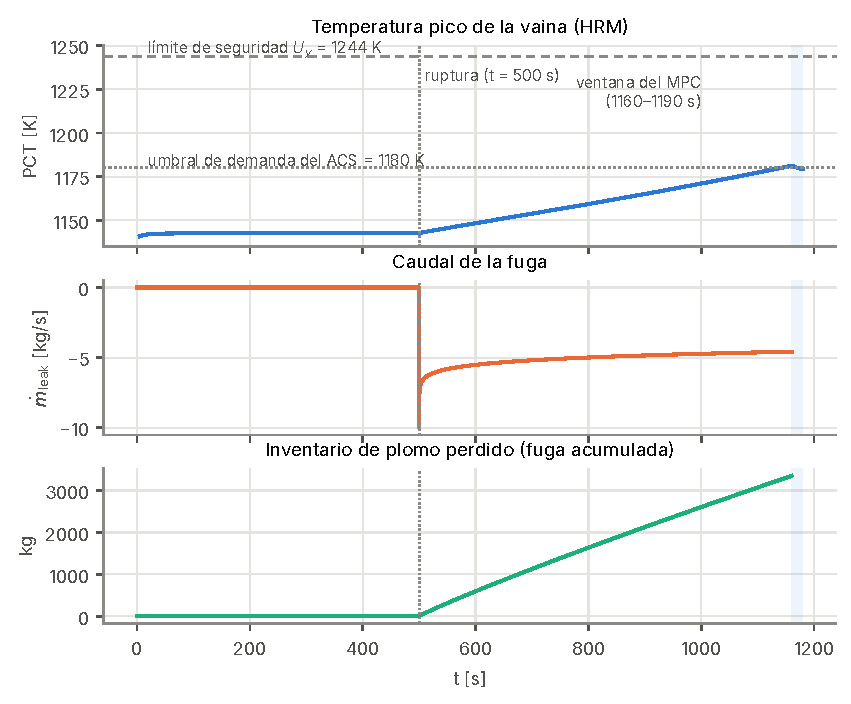
\includegraphics[width=\linewidth]{figures/did_transient.pdf}
\caption{El accidente simulado por el HRM (datos del lazo archivado). Arriba, la PCT; al
medio, el caudal de la fuga; abajo, el plomo perdido, que es la integral de la fuga. La franja
azul marca el periodo en que actúa el controlador. Se omitieron los primeros 5~s (arranque de
la simulación) y una muestra aislada en $t=1160.5$~s, un artefacto del registro al reiniciar
el HRM en la primera consulta. La fuga integrada hasta 1160~s ($-3349$~kg) coincide con el
inventario perdido del estado de la consulta de 1161~s ($-3337$~kg): antes de 1160~s el ACS
no inyectó.}
\label{fig:transitorio}
\end{figure}

\subsection{Por qué sube la PCT: los números}
En la consulta de 1180~s queda el 60\,\% del inventario, así que el caudal primario es
$\mdot_c=0.603\,\mdot_{\rm nom}\approx3349$~kg/s. Esto tiene dos efectos:
\begin{enumerate}
  \item \textbf{El plomo extrae peor el calor de la pared}: $h_{wc}$ cae al
        $0.603^{0.8}\approx67$\,\% de su valor nominal.
  \item \textbf{El plomo se calienta más al atravesar el núcleo}: con una potencia de
        115~MW, el salto de temperatura del refrigerante es
        $P/(\mdot_cc_{p,c})\approx245$~K, frente a 128.5~K en condiciones nominales.
\end{enumerate}
Para devolver el caudal al 80\,\% del nominal habría que reponer unos 1600~kg de plomo. Con el
caudal máximo del ACS, unos 12.9~kg/s, menos la fuga de 4.6~kg/s, eso tomaría unos 190~s:
mucho más que el horizonte de 12.5~s del controlador. Dentro de una consulta, el ACS sólo
puede corregir la PCT en unos pocos kelvin (sección~\ref{sec:autoridad}).

\subsection{El actuador: la bomba magnetohidrodinámica del ACS}
\paragraph{Principio de funcionamiento.} El plomo líquido conduce la electricidad. Una bomba
MHD de conducción hace circular una corriente eléctrica $I$ a través del metal, dentro de un
campo magnético $B$. La fuerza de Lorentz $\mathbf f=\mathbf J\times\mathbf B$ empuja el fluido
sin piezas móviles~\cite{nowak2022}.

\paragraph{El modelo de la bomba.} El proyecto usa un modelo de circuito equivalente (ECM) de
una bomba MHD de corriente continua para el DFR~\cite{nowak2022}:
\[
\Delta P=C\,I-B\,Q-A\,Q^2,
\]
donde $Q$ es el caudal volumétrico. El término $C\,I$ es el empuje de Lorentz; $B\,Q$, las
pérdidas electromagnéticas, que crecen con la velocidad del fluido; y $A\,Q^2$, la fricción
hidráulica. La bomba debe vencer una contrapresión $\Delta P=15$~kPa, así que sólo empieza a
mover plomo cuando $C\,I>\Delta P$, es decir, a partir de $I_0=\Delta P/C=56.687$~A. Por encima
de ese umbral, el caudal másico $\mdot=\rho Q$ crece unos 205~kg/s por cada amperio
(figura~\ref{fig:bomba}).

\begin{figure}[H]\centering
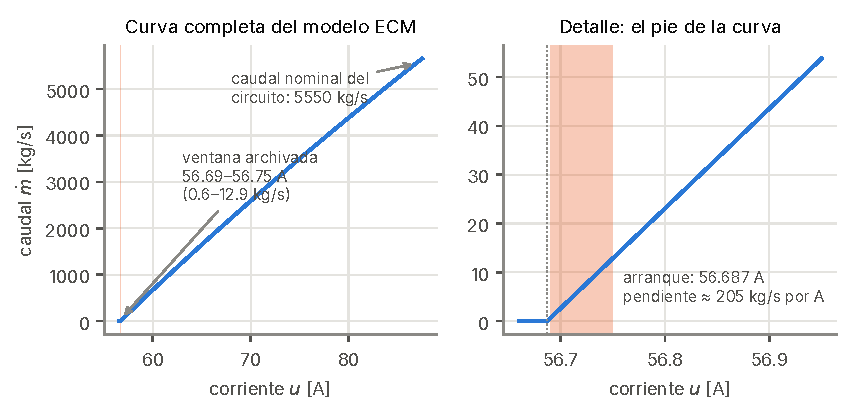
\includegraphics[width=\linewidth]{figures/did_pump.pdf}
\caption{Curva de la bomba MHD según el modelo ECM. Izquierda: la curva completa; el caudal
nominal del circuito primario (5550~kg/s) se alcanza con unos 87~A. Derecha: el detalle del
pie de la curva. La ventana de operación del ACS en el lazo archivado, 56.69--56.75~A
(franja naranja), corresponde a sólo 0.6--12.9~kg/s.}
\label{fig:bomba}
\end{figure}

\noindent La figura deja ver algo importante para el resto del documento. La ventana de
operación del ACS ocupa apenas 0.06~A del pie de una curva que llega a miles de kg/s. Con esa
pendiente, 1~mA de corriente equivale a 0.2~kg/s de caudal. La sección~\ref{sec:actuador}
discute qué significa esto para las cotas del controlador.

\subsection{Variables, límites y referencia}
\begin{table}[H]\centering\small
\begin{tabularx}{\linewidth}{@{}l Y r@{}}\toprule
Magnitud & Significado & Valor\\\midrule
PCT, $\hat y$ & Temperatura pico de la pared de los tubos, estimada por el ROM & $\sim1180$~K\\
$U_y$ & Límite de seguridad de la PCT & 1244~K\\
Umbral de demanda & PCT a partir de la cual se demanda el ACS & 1180~K\\
$y_{\rm ref}$ & Referencia que persigue el controlador (64.7~K bajo el límite) & 1179.27~K\\
$u=\mdot_{\rm ACS}$ & Caudal inyectado por el ACS (la decisión) & 0.58--12.86~kg/s\\
$\Delta t$, $K$ & Paso de decisión y número de pasos del horizonte & 0.5~s, 26\\\bottomrule
\end{tabularx}
\caption{Magnitudes del problema de control.}
\end{table}

\subsection{¿Cuánto puede hacer el actuador en un horizonte?}\label{sec:autoridad}
La figura~\ref{fig:autoridad} responde con el modelo no lineal: simula la PCT durante los
12.5~s del horizonte con cinco caudales constantes del ACS, desde el mínimo hasta el máximo.
Entre el caudal mínimo y el máximo, la PCT al final del horizonte difiere en unos 2.5~K. En
1180~s basta un caudal intermedio para llegar a la referencia. En 1161~s, en cambio, ni
siquiera el caudal máximo alcanza la referencia en 12.5~s: el controlador sólo puede acercar
la PCT, y la mejor decisión es inyectar al máximo.

\begin{figure}[H]\centering
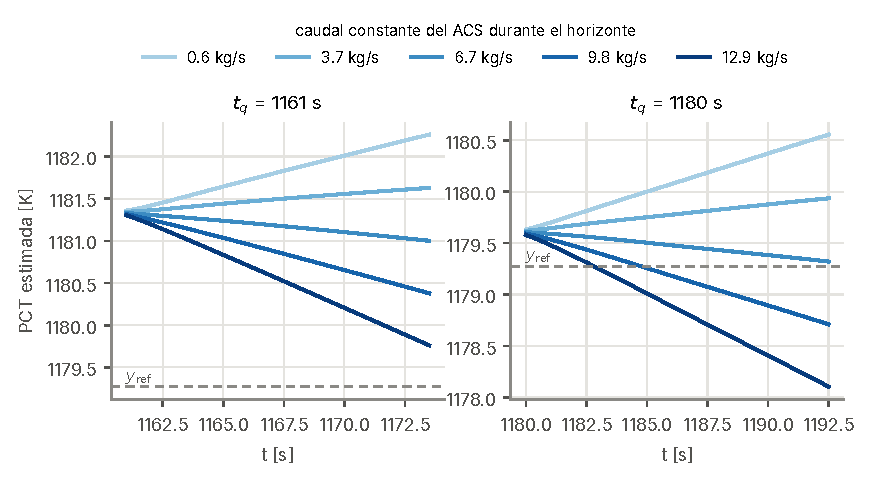
\includegraphics[width=\linewidth]{figures/did_authority.pdf}
\caption{Autoridad del actuador. PCT estimada por el ROM no lineal durante el horizonte, para
cinco caudales constantes del ACS. La diferencia entre el mínimo y el máximo al final del
horizonte es de unos 2.5~K en las dos consultas.}
\label{fig:autoridad}
\end{figure}

\takeaway{\textbf{Para recordar.} En el accidente, la fuga vacía lentamente el circuito
primario y la PCT sube unos 0.06~K/s. El ACS repone plomo, pero su efecto se acumula despacio:
en un horizonte de 12.5~s mueve la PCT sólo unos 2.5~K. Decidir bien cuánto inyectar en cada
instante es justamente el problema del controlador.}
